\chapter{Wyniki i analiza badań}

\section{Wyniki dla modelu uczonego na 25 zdjęciach}

Wykres dokładności modelu, który był uczony na 25 zdjęciach przez 20 epok, prezentuje interesujący profil uczenia się (Rys.~\ref{fig:wykres_dokladnosc_25}). Początkowe wartości dokładności, poniżej 0.7 do 7 epoki, sugerują, że model miał na początku trudności z nauką na dostarczonych danych. Taka sytuacja jest całkiem normalna, zwłaszcza na początku procesu uczenia.

Następnie w epokach od 7 do 15 obserwujemy wahania wartości dokładności, które kształtują się w granicach od 0.7 do 0.9. Ten wzrost i spadek dokładności może świadczyć o tym, że model próbował znaleźć optymalne rozwiązanie w przestrzeni parametrów. Wahania mogą być spowodowane także niewielką ilością danych uczących, co może prowadzić do większej zmienności wyników.

W końcu, wartości dokładności walidacyjnej i testowej są blisko siebie, oscylując między 0.8 a 0.9. To jest dobry znak, sugerujący, że model dobrze się generalizuje i jest w stanie skutecznie przewidywać wyniki na nowych danych. Jednakże, warto pamiętać, że pomimo wysokiej dokładności na końcu, model był uczony na stosunkowo niewielkim zbiorze danych, co może ograniczać jego zdolność do generalizacji na bardziej zróżnicowanych danych.

\begin{figure}[htbp]
  \centering
  \caption{Wykres dokładności dla modelu uczonego na 25 zdjęciach}
  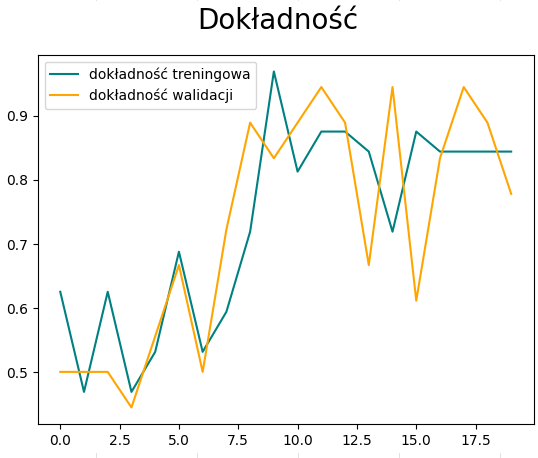
\includegraphics[width=220px]{images/dokladnosc_25.png}
  \begin{center}
  \footnotesize{Źródło: opracowanie własne}
  \end{center}
  \label{fig:wykres_dokladnosc_25}
\end{figure}

\newpage

Wykres straty dla modelu uczonego na 25 zdjęciach przez 20 epok pokazuje, że model poprawiał swoje wyniki na przestrzeni epok, co jest pożądanym zachowaniem (Rys.~\ref{fig:wykres_strata_25}).

Na początku procesu uczenia, strata treningowa zaczęła od wartości 0.8, a następnie skoczyła do 1.8. Strata walidacyjna od początku wynosiła 1.8. Wysokie początkowe wartości straty są typowe dla początkowych etapów uczenia sieci neuronowych. Model na początku jest jeszcze "niewykształcony" i ma tendencję do generowania dużych błędów.

W kolejnych epokach, wartości straty treningowej i walidacyjnej stopniowo malały, co świadczy o tym, że model poprawiał swoją zdolność do prognozowania etykiet w danych treningowych i walidacyjnych. To jest pozytywny wynik, pokazujący, że model uczył się od swoich błędów i poprawiał swoje przewidywania.

Spadek straty w takim samym tępie zarówno dla danych treningowych, jak i walidacyjnych, sugeruje, że model dobrze się generalizuje i nie ma oznak przetrenowania. Przetrenowanie zazwyczaj objawia się dużym spadkiem straty treningowej i niewielkim spadkiem lub nawet wzrostem straty walidacyjnej.

W końcowej, 20 epoce, straty wynosiły poniżej 0.4, co wskazuje na znaczną poprawę w porównaniu do początkowych epok. Jednak nadal jest to stosunkowo wysoka wartość straty i możliwe, że dalsze uczenie lub optymalizacja modelu mogłaby doprowadzić do jej dalszego zmniejszenia.

\begin{figure}[htbp]
  \centering
  \caption{Wykres straty dla modelu uczonego na 25 zdjęciach}
  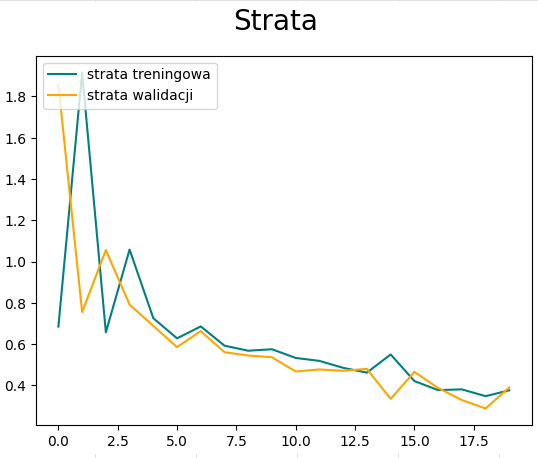
\includegraphics[width=220px]{images/strata_25.png}
  \begin{center}
  \footnotesize{Źródło: opracowanie własne}
  \end{center}
  \label{fig:wykres_strata_25}
\end{figure}

W tabelach zostały przedstawione wyniki testów na zdjęciach z produktami prawidłowymi i uszkodzonymi dla modelu uczonego na 25 zdjęciach. Wartości od 0 do 0.5 zostały przypisane do klasy uszkodzone, a wartości powyżej 0.5 do klasy prawidłowe. Poprawność wyników została oceniona i odpowiednio zapisana. 

Analiza wyników testów dla modelu uczonego na 25 zdjęciach pokazuje, że model osiąga zróżnicowaną skuteczność w ocenie zdjęć z produktami prawidłowymi i uszkodzonymi.

Dla zdjęć z produktami prawidłowymi (Tabela \ref{tab:test_results_prawidlowe_25}), model poprawnie ocenił 9 na 10 przypadków, co daje 90\% skuteczności. Tylko w teście numer 2 model niepoprawnie ocenił element jako "Uszkodzony", gdy był prawidłowy.

W przypadku zdjęć z produktami uszkodzonymi (Tabela \ref{tab:test_results_uszkodzone_25}), model osiągnął niższą skuteczność, poprawnie oceniając 6 na 10 przypadków, co daje 60\% skuteczności. Błędne oceny wystąpiły w testach 1, 3, 6 oraz 10, gdzie model ocenił uszkodzone produkty jako "Prawidłowe".

Ogólna skuteczność modelu uczonego na 25 zdjęciach wynosi 75\% (15 poprawnych ocen na 20 prób). Można zauważyć, że model ma tendencję do lepszego rozpoznawania prawidłowych elementów niż uszkodzonych.

Należy jednak zauważyć, że model był uczony tylko na 25 zdjęciach, co jest stosunkowo małą liczbą przykładów uczących. 

\begin{table}[H]
\centering
\caption{Wyniki testów na zdjęciach z produktami prawidłowymi dla modelu uczonego na 25 zdjęciach}
\begin{tabular}{|c|c|c|c|}
\hline
\textbf{Test} & \textbf{Wynik - Prawidłowe} & \textbf{Ocena} & \textbf{Poprawność oceny} \\ \hline
1  & 0.9185279 & Prawidłowy & Tak \\ \hline
2  & 0.16176112 & Uszkodzony & Nie \\ \hline
3  & 0.84514433 & Prawidłowy & Tak \\ \hline
4  & 0.8351546 & Prawidłowy & Tak \\ \hline
5  & 0.8647871 & Prawidłowy & Tak \\ \hline
6  & 0.72340083 & Prawidłowy & Tak \\ \hline
7  & 0.8165024 & Prawidłowy & Tak \\ \hline
8  & 0.81942993 & Prawidłowy & Tak \\ \hline
9  & 0.7422247 & Prawidłowy & Tak \\ \hline
10 & 0.8814195 & Prawidłowy & Tak \\ \hline
\end{tabular}
\begin{center}
\footnotesize{Źródło: opracowanie własne}
\end{center}
\label{tab:test_results_prawidlowe_25}
\end{table}


\begin{table}[H]
\centering
\caption{Wyniki testów na zdjęciach z produktami uszkodzonymi dla modelu uczonego na 25 zdjęciach}
\begin{tabular}{|c|c|c|c|}
\hline
\textbf{Test} & \textbf{Wynik - Uszkodzone} & \textbf{Ocena} & \textbf{Poprawność oceny}  \\ \hline
1  & 0.54751855 & Prawidłowy & Nie  \\ \hline
2  & 0.24815 & Uszkodzony & Tak \\ \hline
3  & 0.67537665 & Prawidłowy & Nie \\ \hline
4  & 0.2928825 & Uszkodzony & Tak \\ \hline
5  & 0.1816359 & Uszkodzony & Tak \\ \hline
6  & 0.5924341 & Prawidłowy & Nie \\ \hline
7  & 0.33428523 & Uszkodzony & Tak \\ \hline
8  & 0.19617 & Uszkodzony & Tak \\ \hline
9  & 0.25611275 & Uszkodzony & Tak \\ \hline
10 & 0.74181026 & Prawidłowy & Nie \\ \hline
\end{tabular}
\begin{center}
\footnotesize{Źródło: opracowanie własne}
\end{center}
\label{tab:test_results_uszkodzone_25}
\end{table}

\section{Wyniki dla modelu uczonego na 50 zdjęciach}

Wykres dokładności modelu uczonego na 50 zdjęciach przez 20 epok pokazuje ogólnie pozytywną tendencję wzrostu dokładności w czasie treningu (Rys.~\ref{fig:wykres_dokladnosc_50}).

Na początku, wartości dokładności rozpoczęły się na niskim poziomie 0.2. Jest to typowe dla wczesnych etapów uczenia sieci neuronowych, kiedy model nie jest jeszcze w stanie dobrze klasyfikować danych. W kolejnych epokach, dokładność treningowa rosła stopniowo, choć z drobnymi wachaniami.

Między epoką 3 a 5 zaobserwowano istotny wzrost dokładności treningowej, z 0.4 do około 0.8. W kolejnych epokach wachania dokładności treningowej były mniejsze, wynoszące około 0.1.

W przypadku dokładności walidacyjnej, wzrost był bardziej stopniowy, a wachania były mniejsze niż dla dokładności treningowej. To jest pożądane zachowanie, ponieważ oznacza to, że model dobrze generalizuje swoją wiedzę na dane walidacyjne, a nie tylko "zapamiętuje" dane treningowe.

W końcowych epokach, wartości dokładności treningowej i walidacyjnej wachały się między 0.9 a 1. Wysoka dokładność wskazuje, że model jest efektywny w rozpoznawaniu wad produkcyjnych na podstawie dostarczonych danych. Niemniej jednak, warto zwrócić uwagę na możliwość przetrenowania, zwłaszcza gdy dokładność osiąga wartość 1.

\begin{figure}[htbp]
  \centering
  \caption{Wykres dokładności dla modelu uczonego na 50 zdjęciach}
  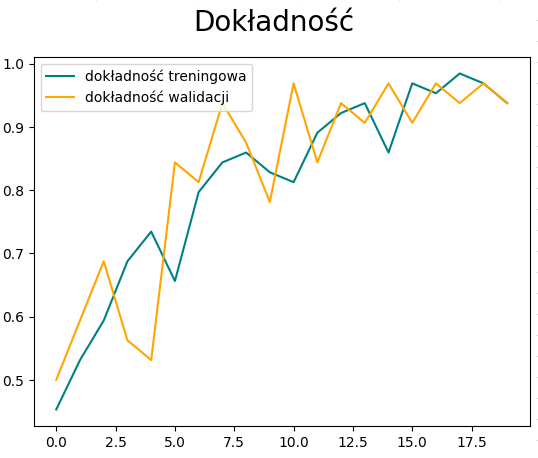
\includegraphics[width=220px]{images/dokladnosc_50.png}
  \begin{center}
  \footnotesize{Źródło: opracowanie własne}
  \end{center}
  \label{fig:wykres_dokladnosc_50}
\end{figure}

Wykres straty modelu uczonego na 50 zdjęciach przez 20 epok pokazuje, że model poprawiał się w trakcie procesu uczenia, co jest zgodne z oczekiwanym zachowaniem (Rys.~\ref{fig:wykres_strata_50}).

Na początku procesu uczenia, wartości straty były dość wysokie, wynosząc około 0.8. Wysoka strata na początku jest typowym zjawiskiem podczas uczenia sieci neuronowych, kiedy model jest jeszcze słabo dopasowany do danych.

Jednakże, z każdą kolejną epoką, wartości straty systematycznie malały. To wskazuje, że model poprawiał swoje predykcje, minimalizując różnice między prognozowanymi a rzeczywistymi etykietami.

Spadek straty był stosunkowo jednolity, co sugeruje, że proces uczenia przebiegał stabilnie. Nie zaobserwowano dużych skoków czy gwałtownych zmian w wartościach straty, co mogłoby sugerować problemy, takie jak zbyt duży współczynnik uczenia.

W końcowej, 20. epoce, wartości straty osiągnęły poziom około 0.1. Jest to znaczne zmniejszenie w porównaniu do początkowych wartości, co sugeruje, że model jest efektywny w rozpoznawaniu wad produkcyjnych na podstawie dostarczonych danych.

Wykres straty pokazuje, że model skutecznie uczył się i poprawiał swoje predykcje w trakcie procesu uczenia. Jednakże, niskie wartości straty na końcu procesu uczenia mogą sugerować, że model jest potencjalnie przetrenowany.

\begin{figure}[htbp]
  \centering
  \caption{Wykres straty dla modelu uczonego na 50 zdjęciach}
  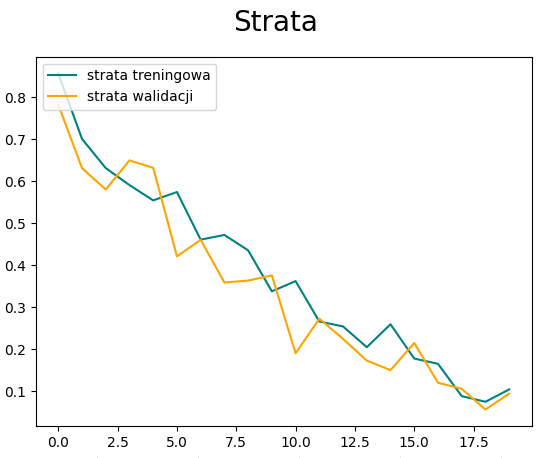
\includegraphics[width=220px]{images/strata_50.png}
  \begin{center}
  \footnotesize{Źródło: opracowanie własne}
  \end{center}
  \label{fig:wykres_strata_50}
\end{figure}

W tabelach zostały przedstawione wyniki testów na zdjęciach z produktami prawidłowymi i uszkodzonymi dla modelu uczonego na 50 zdjęciach. Wartości od 0 do 0.5 zostały przypisane do klasy uszkodzone, a wartości powyżej 0.5 do klasy prawidłowe. Poprawność wyników została oceniona i odpowiednio zapisana.

Analiza wyników testów dla modelu uczonego na 50 zdjęciach pokazuje, że model osiąga lepszą skuteczność w ocenie zdjęć z produktami uszkodzonymi.

Dla zdjęć z produktami prawidłowymi (Tabela \ref{tab:test_results_prawidlowe_50}), model poprawnie ocenił 6 na 10 przypadków, co daje 60\% skuteczności. Błędne oceny wystąpiły w testach 3, 4, 7 i 9 gdzie model niepoprawnie ocenił element jako "Uszkodzony", gdy był prawidłowy.

W przypadku zdjęć z produktami uszkodzonymi (Tabela \ref{tab:test_results_uszkodzone_50}), model osiągnął większą skuteczność niż model uczonego na 25 zdjęciach, poprawnie oceniając 8 na 10 przypadków, co daje 80\% skuteczności. Błędne oceny wystąpiły w testach 1 i 8, gdzie model ocenił uszkodzone produkty jako "Prawidłowe".

Ogólna skuteczność modelu uczonego na 50 zdjęciach wynosi 70\% (14 poprawnych ocen na 20 prób), jest to wyni mniejszy niż dla modelu uczonego na 25 zdjęciach. Jednak warto zauważyć, że model uczonego na 50 zdjęciach osiągnął wyższą skuteczność w ocenie zdjęć z produktami uszkodzonymi.

\begin{table}[H]
\centering
\caption{Wyniki testów na zdjęciach z produktami prawidłowymi dla modelu uczonego na 50 zdjęciach}
\begin{tabular}{|c|c|c|c|}
\hline
\textbf{Test} & \textbf{Wynik} & \textbf{Ocena} & \textbf{Poprawność} \\ \hline
1  & 0.84990263 & Prawidłowy & Tak \\ \hline
2  & 0.9798704 & Prawidłowy & Tak \\ \hline
3  & 0.03639716 & Uszkodzony & Nie \\ \hline
4  & 0.05641427 & Uszkodzony & Nie \\ \hline
5  & 0.9491898 & Prawidłowy & Tak  \\ \hline
6  & 0.7077886 & Prawidłowy & Tak  \\ \hline
7  & 0.2013224 & Uszkodzony & Nie  \\ \hline
8  & 0.88786936 & Prawidłowy & Tak \\ \hline
9  & 0.04853454 & Uszkodzony & Nie \\ \hline
10  & 0.9503239 & Prawidłowy & Tak \\ \hline
\end{tabular}
\begin{center}
\footnotesize{Źródło: opracowanie własne}
\end{center}
\label{tab:test_results_prawidlowe_50}
\end{table}

\begin{table}[H]
\centering
\caption{Wyniki testów na zdjęciach z produktami uszkodzonymi dla modelu uczonego na 50 zdjęciach}
\begin{tabular}{|c|c|c|c|}
\hline
\textbf{Test} & \textbf{Wynik} & \textbf{Ocena} & \textbf{Poprawność} \\ \hline
1  & 0.99400294 & Prawidłowy & Nie \\ \hline
2  & 0.00386766 & Uszkodzony & Tak \\ \hline
3  & 0.01674952 & Uszkodzony & Tak \\ \hline
4  & 0.00414581 & Uszkodzony & Tak \\ \hline
5  & 0.02043912 & Uszkodzony & Tak \\ \hline
6  & 0.00069023 & Uszkodzony & Tak \\ \hline
7  & 0.01667762 & Uszkodzony & Tak \\ \hline
8  & 0.9827842 & Prawidłowy & Nie \\ \hline
9  & 0.01187711 & Uszkodzony & Tak \\ \hline
10  & 0.42052767 & Uszkodzony & Tak \\ \hline
\end{tabular}
\begin{center}
\footnotesize{Źródło: opracowanie własne}
\end{center}
\label{tab:test_results_uszkodzone_50}
\end{table}

\section{Wyniki dla modelu uczonego na 100 zdjęciach}

Wykres dokładności dla modelu uczonego na 100 zdjęciach przez 20 epok pokazuje stopniową poprawę dokładności zarówno na danych treningowych, jak i walidacyjnych w trakcie procesu uczenia (Rys.~\ref{fig:wykres_dokladnosc_100}).

Na początku, dokładność modelu wynosiła około 0.3, co oznacza, że model prawidłowo klasyfikował około 30\% próbek. Stopniowy wzrost dokładności wskazuje na to, że model poprawiał swoje zdolności predykcyjne z każdą kolejną epoką.

Nie zaobserwowano znacznych skoków dokładności, co sugeruje, że proces uczenia przebiegał bez większych problemów. Istotne jest, że dokładność na danych walidacyjnych rosła równomiernie z dokładnością na danych treningowych. To jest dobrym znakiem, ponieważ sugeruje, że model nie był przetrenowany.

W końcowych epokach, dokładność modelu wahała się między 0.8 a 0.9. To oznacza, że model poprawnie klasyfikował około 80-90\% próbek. Jest to dość wysoki poziom dokładności, szczególnie biorąc pod uwagę, że model był uczony na stosunkowo małym zestawie danych.

\begin{figure}[htbp]
  \centering
  \caption{Wykres dokładności dla modelu uczonego na 100 zdjęciach}
  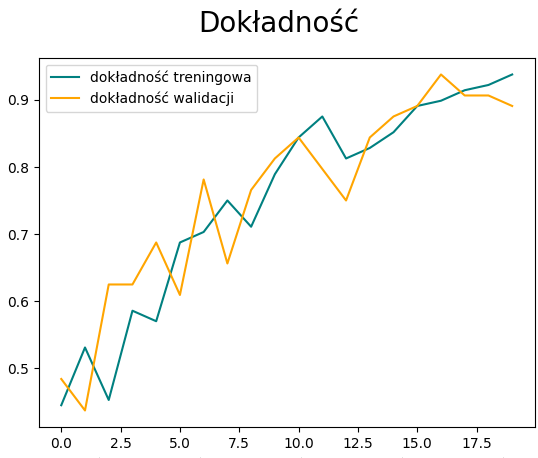
\includegraphics[width=220px]{images/dokladnosc_100.png}
  \begin{center}
  \footnotesize{Źródło: opracowanie własne}
  \end{center}
  \label{fig:wykres_dokladnosc_100}
\end{figure}

Wykres straty dla modelu uczonego na 100 zdjęciach przez 20 epok pokazuje, jak model poprawiał się w trakcie procesu uczenia (Rys.~\ref{fig:wykres_strata_100}). Wysokie początkowe wartości straty (1.6 dla treningowej i 1.3 dla walidacyjnej) wskazują, że na początku procesu uczenia model popełniał wiele błędów w prognozowaniu klas obrazów. To jest spodziewane, ponieważ na początku uczenia, wagi modelu są zazwyczaj inicjalizowane losowo, co prowadzi do losowych prognoz.

Jednak z każdą kolejną epoką, wartości straty zarówno na danych treningowych, jak i walidacyjnych stopniowo malały. To jest dobry znak, ponieważ pokazuje, że model poprawiał swoje zdolności predykcyjne w trakcie uczenia.

Równomierny spadek wartości straty dla danych treningowych i walidacyjnych jest pozytywnym zjawiskiem. Oznacza to, że model był w stanie dobrze generalizować nauczoną wiedzę na nieznane wcześniej dane.

W końcowych epokach, wartości straty wynosiły między 0.4 a 0.2. To oznacza, że model był w stanie poprawnie przewidzieć klasy obrazów z relatywnie niskim błędem.

\begin{figure}[htbp]
  \centering
  \caption{Wykres straty dla modelu uczonego na 100 zdjęciach}
  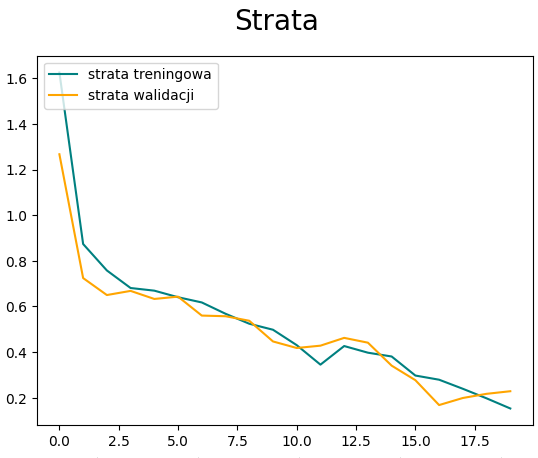
\includegraphics[width=220px]{images/strata_100.png}
  \begin{center}
  \footnotesize{Źródło: opracowanie własne}
  \end{center}
  \label{fig:wykres_strata_100}
\end{figure}

W tabelach zostały przedstawione wyniki testów na zdjęciach z produktami prawidłowymi i uszkodzonymi dla modelu uczonego na 100 zdjęciach. Wartości od 0 do 0.5 zostały przypisane do klasy uszkodzone, a wartości powyżej 0.5 do klasy prawidłowe. Poprawność wyników została oceniona i odpowiednio zapisana.

Analiza wyników testów dla modelu uczonego na 100 zdjęciach pokazuje, że model osiąga lepszą skuteczność w ocenie zdjęć z produktami prawidłowymi niż uszkodzonymi, jednak ogólna skuteczność jest lepsza niż w przypadku modeli uczonych na 25 i 50 zdjęciach.

Dla zdjęć z produktami prawidłowymi (Tabela \ref{tab:test_results_prawidlowe_100}), model poprawnie ocenił 7 na 10 przypadków, co daje 70\% skuteczności. Błędne oceny wystąpiły w testach 6, 7 i 9, gdzie model niepoprawnie ocenił element jako "Uszkodzony", gdy był prawidłowy.

W przypadku zdjęć z produktami uszkodzonymi (Tabela \ref{tab:test_results_uszkodzone_100}), model osiągnął większą skuteczność niż w przypadku modeli uczonych na 25 i 50 zdjęciach, poprawnie oceniając 8 na 10 przypadków, co daje 80\% skuteczności. Błędne oceny wystąpiły w testach 1 i 8, gdzie model ocenił uszkodzone produkty jako "Prawidłowe".

Ogólna skuteczność modelu uczonego na 100 zdjęciach wynosi 75\% (15 poprawnych ocen na 20 prób), tak samo jak dla modelu uczonego na 50 zdjęciach. Jednak warto zauważyć, że model uczonego na 100 zdjęciach osiągnął wyższą skuteczność w ocenie zdjęć z produktami uszkodzonymi niż model uczonego na 25 zdjęciach.

Podobnie jak dla modeli uczonych na mniejszej liczbie zdjęć, zwiększenie liczby zdjęć uczących oraz dalsze strojenie hiperparametrów modelu mogłoby pomóc w poprawie ogólnej skuteczności, szczególnie w rozpoznawaniu uszkodzonych elementów.

\begin{table}[H]
\centering
\caption{Wyniki testów na zdjęciach z produktami prawidłowymi dla modelu uczonego na 100 zdjęciach}
\begin{tabular}{|c|c|c|c|}
\hline
\textbf{Test} & \textbf{Wynik - Prawidłowe} & \textbf{Ocena} & \textbf{Poprawność} \\ \hline
1  & 0.9864047 & Prawidłowy & Tak \\ \hline
2  & 0.812722 & Prawidłowy & Tak \\ \hline
3  & 0.8298837 & Prawidłowy & Tak \\ \hline
4  & 0.8440731 & Prawidłowy & Tak \\ \hline
5  & 0.9554931 & Prawidłowy & Tak \\ \hline
6  & 0.44777694 & Uszkodzony & Nie \\ \hline
7  & 0.2929827 & Uszkodzony & Nie \\ \hline
8  & 0.73627317 & Prawidłowy & Tak \\ \hline
9  & 0.20005107 & Uszkodzony & Nie \\ \hline
10  & 0.94812363 & Prawidłowy & Tak \\ \hline
\end{tabular}
\begin{center}
\footnotesize{Źródło: opracowanie własne}
\end{center}
\label{tab:test_results_prawidlowe_100}
\end{table}

\begin{table}[H]
\centering
\caption{Wyniki testów na zdjęciach z produktami uszkodzonymi dla modelu uczonego na 100 zdjęciach}
\begin{tabular}{|c|c|c|c|}
\hline
\textbf{Test} & \textbf{Wynik - Uszkodzone} & \textbf{Ocena} & \textbf{Poprawność} \\ \hline
1  & 0.9690722 & Prawidłowy & Nie \\ \hline
2  & 0.04128061 & Uszkodzony & Tak \\ \hline
3  & 0.01292709 & Uszkodzony & Tak \\ \hline
4  & 0.01372818 & Uszkodzony & Tak \\ \hline
5  & 0.0035921 & Uszkodzony & Tak \\ \hline
6  & 0.00410713 & Uszkodzony & Tak \\ \hline
7  & 0.09529652 & Uszkodzony & Tak \\ \hline
8  & 0.59629834 & Prawidłowy & Nie \\ \hline
9  & 0.1106549 & Uszkodzony & Tak \\ \hline
10  & 0.40220806 & Uszkodzony & Tak \\ \hline
\end{tabular}
\begin{center}
\footnotesize{Źródło: opracowanie własne}
\end{center}
\label{tab:test_results_uszkodzone_100}
\end{table}

\section{Wyniki dla modelu uczonego na 250 zdjęciach}

Wykres dokładności dla modelu uczonego na 250 zdjęciach pokazuje, że model generalizował dobrze swoją zdolność do klasyfikacji obrazów (Rys.~\ref{fig:wykres_dokladnosc_250}).

Wartości dokładności rozpoczynają się od 0.5 i stopniowo rosną wraz z kolejnymi epokami, co wskazuje na poprawę zdolności klasyfikacyjnych modelu. Wartości dokładności, zarówno dla danych treningowych, jak i walidacyjnych, są do siebie bardzo bliskie przez cały czas uczenia, co jest dobrym znakiem. Oznacza to, że model nie tylko dobrze uczył się na danych treningowych, ale był również w stanie dobrze generalizować nauczoną wiedzę na nieznane wcześniej dane (dane walidacyjne).

Fakt, że wykres ma kształt łyżwy, sugeruje, że model szybko nauczył się klasyfikować obrazy w początkowych epokach, a potem jego dokładność stopniowo się poprawiała, ale w wolniejszym tempie.

W końcowych epokach, wartości dokładności są bardzo blisko 1, co wskazuje na bardzo wysoką zdolność modelu do poprawnej klasyfikacji obrazów. To jest znakomity wynik, który wskazuje na skuteczność zastosowanego podejścia.

\begin{figure}[htbp]
  \centering
  \caption{Wykres dokładności dla modelu uczonego na 250 zdjęciach}
  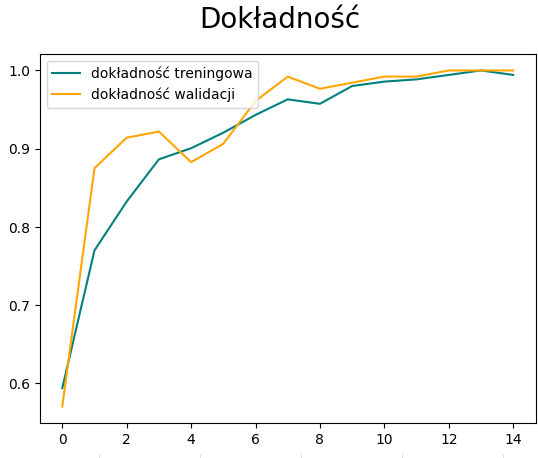
\includegraphics[width=220px]{images/dokladnosc_250.png}
  \begin{center}
  \footnotesize{Źródło: opracowanie własne}
  \end{center}
  \label{fig:wykres_dokladnosc_250}
\end{figure}

Na początku, wartość straty dla zarówno zbioru treningowego jak i walidacyjnego były dość wysokie (0.7 dla treningowego i 0.6 dla walidacyjnego), co jest typowe dla początkowej fazy uczenia modelu (Rys.~\ref{fig:wykres_strata_250}). Jest to oczekiwane, ponieważ model dopiero rozpoczyna uczenie się z danych i jego predykcje są jeszcze dalekie od prawidłowych.

Jednak z każdą kolejną epoką, wartości straty dla obu zestawów danych systematycznie malały, co wskazuje na to, że model poprawiał swoje predykcje. Wartości straty dla danych treningowych i walidacyjnych maleją w podobnym tempie i są bardzo blisko siebie przez cały czas, co jest pozytywnym znakiem. Oznacza to, że model nie tylko dobrze uczył się z danych treningowych, ale również był w stanie skutecznie generalizować swoją wiedzę na nieznane wcześniej dane (dane walidacyjne).

W końcowych epokach, wartości straty są bardzo niskie (między 0.1 a 0), co wskazuje na to, że model jest w stanie dokonywać bardzo precyzyjnych predykcji. Niskie wartości straty na końcu procesu uczenia wskazują na wysoką dokładność modelu.

\begin{figure}[htbp]
  \centering
  \caption{Wykres straty dla modelu uczonego na 250 zdjęciach}
  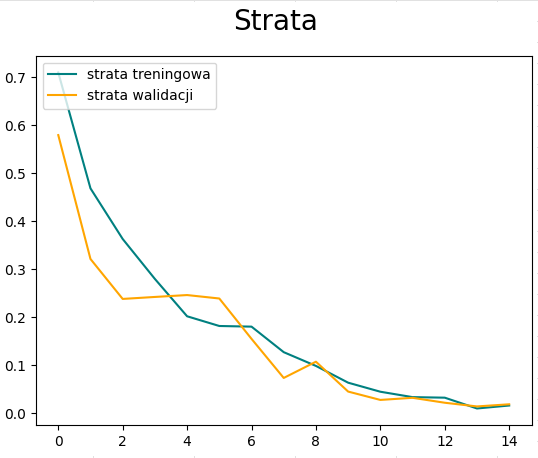
\includegraphics[width=220px]{images/strata_250.png}
  \begin{center}
  \footnotesize{Źródło: opracowanie własne}
  \end{center}
  \label{fig:wykres_strata_250}
\end{figure}

\newpage

W tabelach zostały przedstawione wyniki testów na zdjęciach z produktami prawidłowymi i uszkodzonymi dla modelu uczonego na 250 zdjęciach. Wartości od 0 do 0.5 zostały przypisane do klasy uszkodzone, a wartości powyżej 0.5 do klasy prawidłowe. Poprawność wyników została oceniona i odpowiednio zapisana.

Analiza wyników testów dla modelu uczonego na 250 zdjęciach przez 15 epok pokazuje, że model osiąga lepszą skuteczność w ocenie zdjęć z produktami uszkodzonymi niż prawidłowymi, a ogólna skuteczność jest lepsza niż w przypadku modeli uczonych na 25, 50 i 100 zdjęciach.

Dla zdjęć z produktami prawidłowymi (Tabela \ref{tab:test_results_prawidlowe_250}), model poprawnie ocenił 8 na 10 przypadków, co daje 80\% skuteczności. Błędne oceny wystąpiły w testach 2 i 6, gdzie model niepoprawnie ocenił element jako "Uszkodzony", gdy był prawidłowy.

W przypadku zdjęć z produktami uszkodzonymi (Tabela \ref{tab:test_results_uszkodzone_250}), model osiągnął większą skuteczność niż w przypadku modeli uczonych na 25, 50 i 100 zdjęciach, poprawnie oceniając wszystkie 10 przypadków, co daje 100\% skuteczności.

Ogólna skuteczność modelu uczonego na 250 zdjęciach wynosi 90\% (18 poprawnych ocen na 20 prób), co jest wyższym wynikiem w porównaniu z modelami uczonego na 25, 50 i 100 zdjęciach.

Podobnie jak dla modeli uczonych na mniejszej liczbie zdjęć, zwiększenie liczby zdjęć uczących oraz dalsze strojenie hiperparametrów modelu mogłoby pomóc w poprawie ogólnej skuteczności, szczególnie w rozpoznawaniu prawidłowych elementów.

\begin{table}[H]
\centering
\caption{Wyniki testów na zdjęciach z produktami prawidłowymi na 250 zdjęciach}
\begin{tabular}{|c|c|c|c|}
\hline
\textbf{Test} & \textbf{Wynik - Prawidłowe} & \textbf{Ocena} & \textbf{Poprawność} \\ \hline
1  & 0.99992514 & Prawidłowy & Tak \\ \hline
2  & 0.00049097 & Uszkodzony & Nie \\ \hline
3  & 0.99903715 & Prawidłowy & Tak \\ \hline
4  & 0.9983879 & Prawidłowy & Tak \\ \hline
5  & 0.97826487 & Prawidłowy & Tak \\ \hline
6  & 0.2164898 & Uszkodzony & Nie \\ \hline
7  & 0.9998957 & Prawidłowy & Tak \\ \hline
8  & 0.99057996 & Prawidłowy & Tak \\ \hline
9  & 0.7195368 & Prawidłowy & Tak \\ \hline
10  & 0.9921462 & Prawidłowy & Tak \\ \hline
\end{tabular}
\begin{center}
\footnotesize{Źródło: opracowanie własne}
\end{center}
\label{tab:test_results_prawidlowe_250}
\end{table}

\begin{table}[H]
\centering
\caption{Wyniki testów na zdjęciach z produktami uszkodzonymi na 250 zdjęciach}
\begin{tabular}{|c|c|c|c|}
\hline
\textbf{Test} & \textbf{Wynik - Uszkodzone} & \textbf{Ocena} & \textbf{Poprawność} \\ \hline
1  & 0.14923318 & Uszkodzony & Tak \\ \hline
2  & 2.871099e-08 & Uszkodzony & Tak \\ \hline
3  & 9.253375e-05 & Uszkodzony & Tak \\ \hline
4  & 4.3932796e-06 & Uszkodzony & Tak \\ \hline
5  & 1.2867513e-08 & Uszkodzony & Tak \\ \hline
6  & 1.791459e-08 & Uszkodzony & Tak \\ \hline
7  & 0.00028085 & Uszkodzony & Tak \\ \hline
8  & 0.00098794 & Uszkodzony & Tak \\ \hline
9  & 2.8661802e-06 & Uszkodzony & Tak \\ \hline
10  & 0.00594379 & Uszkodzony & Tak \\ \hline
\end{tabular}
\begin{center}
\footnotesize{Źródło: opracowanie własne}
\end{center}
\label{tab:test_results_uszkodzone_250}
\end{table}

\section{Wyniki dla modelu uczonego na 500 zdjęciach}

Wykres dokładności modelu, który był trenowany na 500 zdjęciach przez 15 epok, wskazuje na bardzo dobrą zdolność modelu do klasyfikacji obrazów (Rys.~\ref{fig:wykres_dokladnosc_500}).

Na początku procesu uczenia, dokładność dla danych treningowych wynosiła 0.7, natomiast dla danych walidacyjnych - 0.89. Różnica między nimi może wynikać z różnic w dystrybucji danych, jednak obie wartości są dość wysokie już na tym etapie, co sugeruje, że model już na początku był w stanie dobrze klasyfikować obrazy.

W miarę postępu procesu uczenia, dokładność modelu na danych treningowych i walidacyjnych stale rosła, co jest oznaką skutecznego uczenia. Warto zauważyć, że pomimo drobnych wahań, ogólny trend wzrostowy był konsekwentny i stopniowy, bez znacznych skoków, co wskazuje na stabilność procesu uczenia.

W końcowych epokach, dokładność modelu na danych treningowych zbliżała się do 1, co oznacza, że model prawie idealnie klasyfikował obrazy z zestawu treningowego. Dokładność na danych walidacyjnych wynosiła 0.95, co jest również bardzo wysokim wynikiem i sugeruje, że model dobrze generalizuje swoją wiedzę na nowe, nieznane wcześniej dane.

\begin{figure}[htbp]
  \centering
  \caption{Wykres dokładności dla modelu uczonego na 500 zdjęciach}
  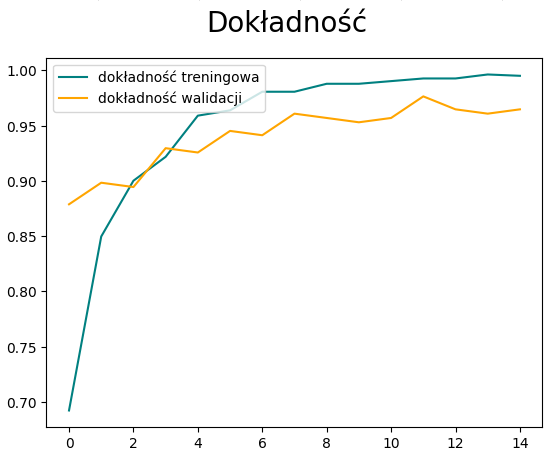
\includegraphics[width=220px]{images/dokladnosc_500.png}
  \begin{center}
  \footnotesize{Źródło: opracowanie własne}
  \end{center}
  \label{fig:wykres_dokladnosc_500}
\end{figure}

Wykres straty modelu, który był trenowany na 500 zdjęciach przez 15 epok, wskazuje na efektywny proces uczenia (Rys.~\ref{fig:wykres_strata_500}).

Na początku procesu uczenia, strata dla danych treningowych wynosiła 0.7, natomiast dla danych walidacyjnych - 0.4. Ta różnica może wynikać z różnic w dystrybucji danych między zestawem treningowym i walidacyjnym. Warto zauważyć, że pomimo tej różnicy, wartości straty były na akceptowalnym poziomie już na początku procesu uczenia, co sugeruje, że model już na tym etapie był w stanie dość dobrze klasyfikować obrazy.

W miarę postępu procesu uczenia, strata modelu na danych treningowych i walidacyjnych stale malała, co jest oznaką skutecznego uczenia. Ogólny trend spadkowy był konsekwentny i stopniowy, co wskazuje na stabilność procesu uczenia.

W końcowych epokach, strata modelu na danych treningowych zbliżała się do 0, co oznacza, że model prawie idealnie klasyfikował obrazy z zestawu treningowego. Strata na danych walidacyjnych wynosiła 0.2, co jest również niskim wynikiem i sugeruje, że model dobrze generalizuje swoją wiedzę na nowe, nieznane wcześniej dane.

\begin{figure}[htbp]
  \centering
  \caption{Wykres straty dla modelu uczonego na 500 zdjęciach}
  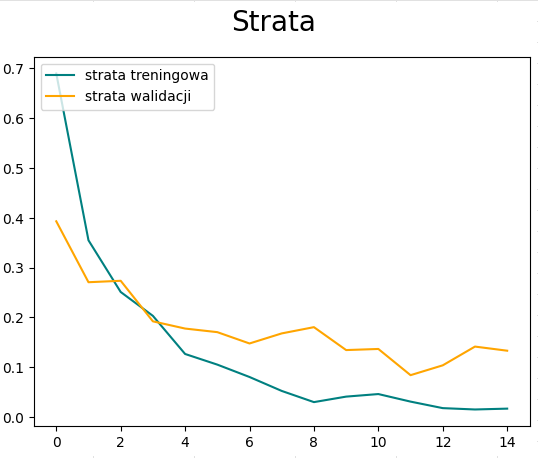
\includegraphics[width=220px]{images/strata_500.png}
  \begin{center}
  \footnotesize{Źródło: opracowanie własne}
  \end{center}
  \label{fig:wykres_strata_500}
\end{figure}

W tabelach zostały przedstawione wyniki testów na zdjęciach z produktami prawidłowymi i uszkodzonymi dla modelu uczonego na 500 zdjęciach. Wartości od 0 do 0.5 zostały przypisane do klasy uszkodzone, a wartości powyżej 0.5 do klasy prawidłowe. Poprawność wyników została oceniona i odpowiednio zapisana.

Analiza wyników testów dla modelu uczonego na 500 zdjęciach pokazuje, że model osiąga znakomitą skuteczność w ocenie zdjęć zarówno z produktami prawidłowymi, jak i uszkodzonymi. Ogólna skuteczność jest znacznie lepsza niż w przypadku modeli uczonych na 25, 50, 100 i 250 zdjęciach.

Dla zdjęć z produktami prawidłowymi (Tabela \ref{tab:test_results_prawidlowe_500}), model poprawnie ocenił wszystkie 10 przypadków, co daje 100\% skuteczności. Nie wystąpiły żadne błędne oceny.

W przypadku zdjęć z produktami uszkodzonymi (Tabela \ref{tab:test_results_uszkodzone_500}), model również osiągnął 100\% skuteczność, poprawnie oceniając wszystkie 10 przypadków. Nie wystąpiły żadne błędne oceny.

Ogólna skuteczność modelu uczonego na 500 zdjęciach wynosi 100\% (20 poprawnych ocen na 20 prób), co jest znacznie wyższym wynikiem w porównaniu z modelami uczonymi na 25, 50, 100 i 250 zdjęciach.

Wyniki te wskazują, że zwiększenie liczby zdjęć uczących oraz dalsze strojenie hiperparametrów modelu przyczyniło się do znaczącej poprawy ogólnej skuteczności. 

\begin{table}[H]
\centering
\caption{Wyniki testów na zdjęciach z produktami prawidłowymi dla modelu uczonego na 500 zdjęciach}
\begin{tabular}{|c|c|c|c|}
\hline
\textbf{Test} & \textbf{Wynik - Prawidłowe} & \textbf{Ocena} & \textbf{Poprawny} \\ \hline
1  & 0.99994624 & Prawidłowy & Tak  \\ \hline
2  & 0.86573 & Prawidłowy & Tak \\ \hline
3  & 0.99992496 & Prawidłowy & Tak \\ \hline
4  & 0.99304414 & Prawidłowy & Tak \\ \hline
5  & 0.9994097 & Prawidłowy & Tak \\ \hline
6  & 0.74320 & Prawidłowy & Tak  \\ \hline
7  & 0.99879295 & Prawidłowy & Tak  \\ \hline
8  & 0.98510396 & Prawidłowy & Tak \\ \hline
9  & 0.9975974 & Prawidłowy & Tak \\ \hline
10  & 0.9990083 & Prawidłowy & Tak \\ \hline
\end{tabular}
\begin{center}
\footnotesize{Źródło: opracowanie własne}
\end{center}
\label{tab:test_results_prawidlowe_500}
\end{table}

\begin{table}[H]
\centering
\caption{Wyniki testów na zdjęciach z produktami uszkodzonymi dla modelu uczonego na 500 zdjęciach}
\begin{tabular}{|c|c|c|c|}
\hline
\textbf{Test} & \textbf{Wynik - Uszkodzone} & \textbf{Ocena} & \textbf{Poprawny} \\ \hline
1  & 7.884345e-05 & Uszkodzony & Tak  \\ \hline
2  & 4.773199e-07 & Uszkodzony & Tak \\ \hline
3  & 2.2078943e-06 & Uszkodzony & Tak \\ \hline
4  & 6.3885636e-06 & Uszkodzony & Tak \\ \hline
5  & 9.216427e-06 & Uszkodzony & Tak \\ \hline
6  & 2.3838764e-09 & Uszkodzony & Tak  \\ \hline
7  & 1.6288888e-07 & Uszkodzony & Tak \\ \hline
8 & 0.00364679 & Uszkodzony & Tak \\ \hline
9 & 9.597346e-06 & Uszkodzony & Tak \\ \hline
10 & 0.00247978 & Uszkodzony & Tak \\ \hline
\end{tabular}
\begin{center}
\footnotesize{Źródło: opracowanie własne}
\end{center}
\label{tab:test_results_uszkodzone_500}
\end{table}

\section{Podsumowanie wyników}

Wyniki badań wskazują, że jakość modelu ulega poprawie wraz ze wzrostem liczby zdjęć wykorzystanych do treningu (Tabela \ref{tab:test_results_summary}). Model trenowany na 25 zdjęciach osiąga poprawność na poziomie 75\%, natomiast model trenowany na 50 zdjęciach uzyskuje nieco niższą poprawność wynoszącą 70\%. W przypadku modelu trenowanego na 100 zdjęciach poprawność wynosi 75\%. Liczba zdjęć wykorzystana podczas tych badań była niska, dlatego też można zauważyć, że oceny w tych modelach były niestabilne. W przypadku modelu trenowanego na 25 zdjęciach, model miał tendencje do lepszego rozpoznawania prawidłowych elementów. Natomiast w przypadku modelu trenowanego na 50 zdjęciach model lepiej rozpoznawał uszkodzone elementy.

Znacząca poprawa wydajności modelu następuje przy zastosowaniu 250 zdjęć do treningu, gdzie poprawność wynosi 90\%. Ostatecznie, model trenowany na 500 zdjęciach osiąga 100\% poprawności, co świadczy o dobrej zdolności do klasyfikacji zdjęć.

Wnioskiem z przeprowadzonych testów jest zatem to, że większa liczba zdjęć użytych do treningu skutkuje lepszymi wynikami modelu. Warto zwrócić uwagę na korzyści płynące z zastosowania większego zbioru danych, szczególnie gdy dąży się do uzyskania wysokiej poprawności klasyfikacji.

\begin{table}[H]
\centering
\caption{Podsumowanie wyników testów}
\begin{tabular}{|c|c|c|c|c|}
\hline
\textbf{Model} & \textbf{Liczba zdjęć} & \textbf{Prawidłowe} & \textbf{Uszkodzone} & \textbf{Poprawność [\%]} \\ \hline
25 zdjęć & 20 & 9 & 6 & 75 \\ \hline
50 zdjęć & 20 & 6 & 8 & 70 \\ \hline
100 zdjęć & 20 & 7 & 8 & 75 \\ \hline
250 zdjęć & 20 & 8 & 10 & 90 \\ \hline
500 zdjęć & 20 & 10 & 10 & 100 \\ \hline
\end{tabular}
\begin{center}
\footnotesize{Źródło: opracowanie własne}
\end{center}
\label{tab:test_results_summary}
\end{table}